\subsubsection{Statistical Physics of Biological Networks}
\index{Meyer-Ortmanns, Hildegard}

\paragraph{Research Team} Hildegard Meyer-Ortmanns (Professor), Xiang Li (Humboldt Fellow),
Filippo Radicchi (Research Associate), Daniele Vilone
(Postdoctoral Fellow), Sooyeon Yoon (Visiting Graduate Student), Yeong-Yeol Ahn (Visiting Graduate Student)\\

Biological networks are naturally occurring systems of interacting
units. The units are assigned to the nodes such as genes, proteins, metabolites, or neurons,
while regulating relations between the genes or the
proteins, chemical reactions between metabolites, or
synaptic connections between the neurons are assigned to the edges of
the network. A number of models is used to describe various
dynamical aspects. One of these models are Boolean networks that were introduced
by Stuart Kauffman in 1969 as a simple model for genetic systems.\\
A topical issue in the context of genetic networks is an
explanation of the low number of stable cell states in spite of the fact that
many states are in principle possible if all combinations of
genes would be allowed. Boolean dynamics may result in a limited
number of attractors in phase space and - if attractors actually represent cell states- Boolean
dynamics would explain
the observation of a few stable cell states. Random Boolean networks are directed
graphs with $N$ nodes each of which takes a Boolean value $0$ or $1$.
Usually the nodes are synchronously updated from time $t$ to time
$t+1$ according to coupling functions that are chosen randomly
from a certain set of Boolean functions. As it turned out, the
increase of the number of stable attractors as a function of the
system size does depend on the updating mode, being
synchronous or asynchronous. An exponential growth of the
number of attractors with the system size seems to be an artifact of the
synchronous update which is not realistic from the biological
point of view.

\paragraph{Highlights}
%
\textit{Synchronous versus asynchronous update}
We have started with a systematic study of synchronous versus
asynchronous updating modes, first applied to an Ising chain in
which each unit can take only two possible values, $+1$ or $-1$.
Already in this simple system we observe a phase transition
between the stationary states of the time evolution
\cite{meyerortmanns1} if we interpolate between synchronous and
asynchronous updating. (Interestingly for physicists: this
transition belongs to the universality class of parity
conservation.) In general, the effect of such a transition may be
that in one of these phases the stationary states have lost any
remnants to the intrinsic dynamics that was imposed on the
individual nodes of the network. In this case the stationary
states are no longer representative for a certain intrinsic
dynamics, but depend on the time-order of updating events.
In turn this has an impact on the interpretation of datasets
as reflecting certain intrinsic dynamics.\\

\begin{figure}[ht]
  \begin{center}
    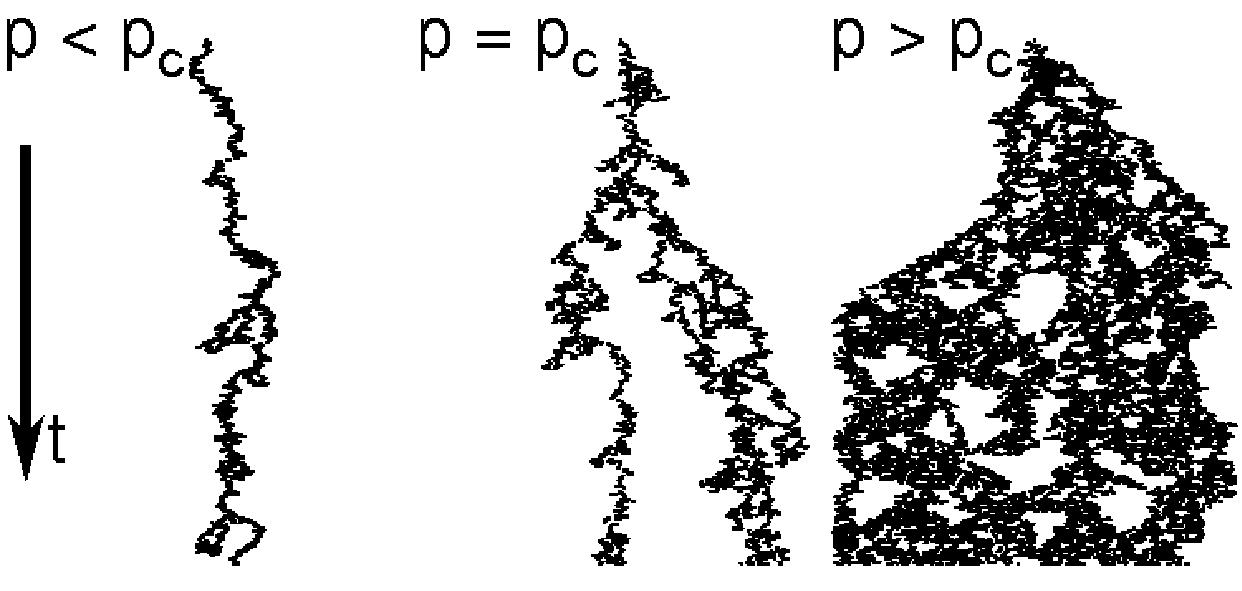
\includegraphics[width=\hsize]{Meyer-Ortmanns/meyerortmanns.pdf}
    \mycaption{Directed percolation process in time as it also occurs for processes of epidemic spreading.
$p_c$ is a critical parameter beyond which the qualitative behavior changes.}\label{fig:meyerortmanns1}
   \end{center}
\end{figure}

We will generalize the dynamics and vary the updating rules to
biologically more relevant ones. In this way we can check which
features of the space of attractors depend on the used procedures
and how the number of stable cell states is influenced by the
order of updating events. \newline \newline Hildegard Meyer-Ortmanns is also involved in ``Statistical Physics: Dynamical Processes on Complex
Networks''.


\paragraph{Organization}
\begin{enumerate}
\item  ICTS-seminars 2006
\end{enumerate}

\myparagraph{Collaborations}
%
Bremen Area Collaborations:
\begin{enumerate}
\item {\sl International University Bremen}\\Prof. M.-Th. H\"utt\\Genetic Networks
\\Prof. C. Hilgetag\\Neural Networks
\item {\sl Bremen University} \\Prof. S. Bornholdt\\Boolean Networks
\end{enumerate}

National \& International Collaborations:
\begin{enumerate}
\item {\sl Kyung Hee University, Seoul (Korea)}\\ Prof. S.-H.
Yook\\ Percolation theory and epidemic spreading
\item{\sl Korea Institute of Advanced Science and Technology, Daejeon,
Korea}\\Y.Y. Ahn\\ Neural Network Models for the Visual
Cortex of the Monkey
\item{\sl Humboldt University Berlin}\\Prof. M. Zaks\\ Dynamics of Excitable Media
\item {\sl Technische Universit\"at Hamburg Harburg}\\ Prof. A.-P. Zeng\\ Autocatalytic Sets and Metabolic Networks
\end{enumerate}


\paragraph{Grants}
\begin{enumerate}
\item Funded by DFG,  \emph{Hierarchische Netzwerke}, ME
1332/10-2, (April 2004 - March 2007)
\end{enumerate}

\paragraph{Other Support Grants}
\begin{enumerate}
\item Humboldt-Stiftung, Fellowship, Humboldt-Stiftung
IV-CHN/1116658 STP
\item 2 DAAD-grants (Germany-Korea): a) ``Physics of Surface Growth'', b) ``Neural Networks''
\end{enumerate}


\paragraph{Awards, Prizes}
\begin{enumerate}
\item W.E. Heraeus summer school on {\it Interfaces between Physics
and Computer Science} to take place in June 2007, approved in 2006
\item W.E. Heraeus summer school on {\it Statistical Physics of
Gene Regulation: From Genetic Networks to Expression Data and Back
} (organized with M.T. H\"utt) to take place in July 2007, approved
in 2006
\end{enumerate}

\nocite{ortmanns0M}
\nocite{ortmanns1M}
\nocite{ortmanns2M}
\nocite{ortmanns3M}
\nocite{ortmanns4M}
\nocite{ortmanns5M}
\nocite{ortmanns6M}
%\nocite{meyerortmanns1M}
\nocite{vilone1M}
